\documentclass[]{article}
\usepackage{lmodern}
\usepackage{amssymb,amsmath}
\usepackage{ifxetex,ifluatex}
\usepackage{fixltx2e} % provides \textsubscript
\ifnum 0\ifxetex 1\fi\ifluatex 1\fi=0 % if pdftex
  \usepackage[T1]{fontenc}
  \usepackage[utf8]{inputenc}
\else % if luatex or xelatex
  \ifxetex
    \usepackage{mathspec}
  \else
    \usepackage{fontspec}
  \fi
  \defaultfontfeatures{Ligatures=TeX,Scale=MatchLowercase}
\fi
% use upquote if available, for straight quotes in verbatim environments
\IfFileExists{upquote.sty}{\usepackage{upquote}}{}
% use microtype if available
\IfFileExists{microtype.sty}{%
\usepackage{microtype}
\UseMicrotypeSet[protrusion]{basicmath} % disable protrusion for tt fonts
}{}
\usepackage[margin=1in]{geometry}
\usepackage{hyperref}
\hypersetup{unicode=true,
            pdfborder={0 0 0},
            breaklinks=true}
\urlstyle{same}  % don't use monospace font for urls
\usepackage{color}
\usepackage{fancyvrb}
\newcommand{\VerbBar}{|}
\newcommand{\VERB}{\Verb[commandchars=\\\{\}]}
\DefineVerbatimEnvironment{Highlighting}{Verbatim}{commandchars=\\\{\}}
% Add ',fontsize=\small' for more characters per line
\usepackage{framed}
\definecolor{shadecolor}{RGB}{248,248,248}
\newenvironment{Shaded}{\begin{snugshade}}{\end{snugshade}}
\newcommand{\KeywordTok}[1]{\textcolor[rgb]{0.13,0.29,0.53}{\textbf{#1}}}
\newcommand{\DataTypeTok}[1]{\textcolor[rgb]{0.13,0.29,0.53}{#1}}
\newcommand{\DecValTok}[1]{\textcolor[rgb]{0.00,0.00,0.81}{#1}}
\newcommand{\BaseNTok}[1]{\textcolor[rgb]{0.00,0.00,0.81}{#1}}
\newcommand{\FloatTok}[1]{\textcolor[rgb]{0.00,0.00,0.81}{#1}}
\newcommand{\ConstantTok}[1]{\textcolor[rgb]{0.00,0.00,0.00}{#1}}
\newcommand{\CharTok}[1]{\textcolor[rgb]{0.31,0.60,0.02}{#1}}
\newcommand{\SpecialCharTok}[1]{\textcolor[rgb]{0.00,0.00,0.00}{#1}}
\newcommand{\StringTok}[1]{\textcolor[rgb]{0.31,0.60,0.02}{#1}}
\newcommand{\VerbatimStringTok}[1]{\textcolor[rgb]{0.31,0.60,0.02}{#1}}
\newcommand{\SpecialStringTok}[1]{\textcolor[rgb]{0.31,0.60,0.02}{#1}}
\newcommand{\ImportTok}[1]{#1}
\newcommand{\CommentTok}[1]{\textcolor[rgb]{0.56,0.35,0.01}{\textit{#1}}}
\newcommand{\DocumentationTok}[1]{\textcolor[rgb]{0.56,0.35,0.01}{\textbf{\textit{#1}}}}
\newcommand{\AnnotationTok}[1]{\textcolor[rgb]{0.56,0.35,0.01}{\textbf{\textit{#1}}}}
\newcommand{\CommentVarTok}[1]{\textcolor[rgb]{0.56,0.35,0.01}{\textbf{\textit{#1}}}}
\newcommand{\OtherTok}[1]{\textcolor[rgb]{0.56,0.35,0.01}{#1}}
\newcommand{\FunctionTok}[1]{\textcolor[rgb]{0.00,0.00,0.00}{#1}}
\newcommand{\VariableTok}[1]{\textcolor[rgb]{0.00,0.00,0.00}{#1}}
\newcommand{\ControlFlowTok}[1]{\textcolor[rgb]{0.13,0.29,0.53}{\textbf{#1}}}
\newcommand{\OperatorTok}[1]{\textcolor[rgb]{0.81,0.36,0.00}{\textbf{#1}}}
\newcommand{\BuiltInTok}[1]{#1}
\newcommand{\ExtensionTok}[1]{#1}
\newcommand{\PreprocessorTok}[1]{\textcolor[rgb]{0.56,0.35,0.01}{\textit{#1}}}
\newcommand{\AttributeTok}[1]{\textcolor[rgb]{0.77,0.63,0.00}{#1}}
\newcommand{\RegionMarkerTok}[1]{#1}
\newcommand{\InformationTok}[1]{\textcolor[rgb]{0.56,0.35,0.01}{\textbf{\textit{#1}}}}
\newcommand{\WarningTok}[1]{\textcolor[rgb]{0.56,0.35,0.01}{\textbf{\textit{#1}}}}
\newcommand{\AlertTok}[1]{\textcolor[rgb]{0.94,0.16,0.16}{#1}}
\newcommand{\ErrorTok}[1]{\textcolor[rgb]{0.64,0.00,0.00}{\textbf{#1}}}
\newcommand{\NormalTok}[1]{#1}
\usepackage{graphicx,grffile}
\makeatletter
\def\maxwidth{\ifdim\Gin@nat@width>\linewidth\linewidth\else\Gin@nat@width\fi}
\def\maxheight{\ifdim\Gin@nat@height>\textheight\textheight\else\Gin@nat@height\fi}
\makeatother
% Scale images if necessary, so that they will not overflow the page
% margins by default, and it is still possible to overwrite the defaults
% using explicit options in \includegraphics[width, height, ...]{}
\setkeys{Gin}{width=\maxwidth,height=\maxheight,keepaspectratio}
\IfFileExists{parskip.sty}{%
\usepackage{parskip}
}{% else
\setlength{\parindent}{0pt}
\setlength{\parskip}{6pt plus 2pt minus 1pt}
}
\setlength{\emergencystretch}{3em}  % prevent overfull lines
\providecommand{\tightlist}{%
  \setlength{\itemsep}{0pt}\setlength{\parskip}{0pt}}
\setcounter{secnumdepth}{0}
% Redefines (sub)paragraphs to behave more like sections
\ifx\paragraph\undefined\else
\let\oldparagraph\paragraph
\renewcommand{\paragraph}[1]{\oldparagraph{#1}\mbox{}}
\fi
\ifx\subparagraph\undefined\else
\let\oldsubparagraph\subparagraph
\renewcommand{\subparagraph}[1]{\oldsubparagraph{#1}\mbox{}}
\fi

%%% Use protect on footnotes to avoid problems with footnotes in titles
\let\rmarkdownfootnote\footnote%
\def\footnote{\protect\rmarkdownfootnote}

%%% Change title format to be more compact
\usepackage{titling}

% Create subtitle command for use in maketitle
\newcommand{\subtitle}[1]{
  \posttitle{
    \begin{center}\large#1\end{center}
    }
}

\setlength{\droptitle}{-2em}

  \title{}
    \pretitle{\vspace{\droptitle}}
  \posttitle{}
    \author{}
    \preauthor{}\postauthor{}
    \date{}
    \predate{}\postdate{}
  
\usepackage{float}

\begin{document}

\begin{centering}

\vspace*{5 cm}

\Huge

{\bf Descubrimiento del Conocimiento usando herramientas de Big Data Módulo 2}

\vspace{3 cm}

\Large
Marco Andrés Vázquez Hernández

\vspace{1 cm}
\normalsize
Práctica de Regresion Logística. 

Septiembre de 2018

\normalsize
Instituto Politécnico Nacional


\end{centering}

\newpage

\section{Descripción}\label{descripcion}

1- Encontrar las variables que generen una mayor exactitud (accuracy)
del conjunto de datos anterior. 2- Documentar el procedmiento. 3-
Realizar el preprocesamiento de datos en caso de ser necesario.

\section{Integración de los archivos}\label{integracion-de-los-archivos}

Se cargaron los datos y se separaron las variables: Obs.No se elimina y
se separa ``Buy'' dado que es la variable que queremos explicar.

\begin{Shaded}
\begin{Highlighting}[]
\ImportTok{from}\NormalTok{ sklearn }\ImportTok{import}\NormalTok{ linear_model}
\ImportTok{from}\NormalTok{ sklearn }\ImportTok{import}\NormalTok{ preprocessing}
\ImportTok{import}\NormalTok{ numpy }\ImportTok{as}\NormalTok{ np}
\ImportTok{import}\NormalTok{ pandas }\ImportTok{as}\NormalTok{ pd}
\ImportTok{import}\NormalTok{ matplotlib}
\ImportTok{import}\NormalTok{ matplotlib.pyplot }\ImportTok{as}\NormalTok{ plt}
\ImportTok{import}\NormalTok{ scipy.stats }\ImportTok{as}\NormalTok{ stats}
\ImportTok{import}\NormalTok{ itertools}
\NormalTok{dataPeople }\OperatorTok{=}\NormalTok{ pd.read_csv(}\StringTok{"clientes.csv"}\NormalTok{)}
\NormalTok{lst }\OperatorTok{=}\NormalTok{ dataPeople.columns}
\NormalTok{no_lst }\OperatorTok{=}\NormalTok{ [}\StringTok{'Obs No.'}\NormalTok{,}\StringTok{'Buy'}\NormalTok{]}
\end{Highlighting}
\end{Shaded}

Se hicieron dos loops for: 1.- El primero corre en la variable ``j'' de
0 hasta el máximo de variables en lst -1 ya que hace uso de la función
itertools.combinations que arroja una lista de todas las combinaciónes
de tamaño j.

2.- Después se corre y compara la accuracy de cada una de las
combinaciones de tamaño j y se guarda la combinación con mayor accuracy.

\begin{Shaded}
\begin{Highlighting}[]
\NormalTok{aux_acc}\OperatorTok{=}\DecValTok{0}
\BuiltInTok{print}\NormalTok{(}\BuiltInTok{range}\NormalTok{(}\BuiltInTok{len}\NormalTok{(lst)))}
\ControlFlowTok{for}\NormalTok{ j }\KeywordTok{in} \BuiltInTok{range}\NormalTok{(}\BuiltInTok{len}\NormalTok{(lst)}\OperatorTok{-}\DecValTok{1}\NormalTok{):}
    \BuiltInTok{print}\NormalTok{ (j)}
\NormalTok{    combinaciones }\OperatorTok{=} \BuiltInTok{list}\NormalTok{(itertools.combinations([c }\ControlFlowTok{for}\NormalTok{ c }\KeywordTok{in}\NormalTok{ dataPeople.columns }\ControlFlowTok{if}\NormalTok{ c }\KeywordTok{not} \KeywordTok{in}\NormalTok{ no_lst], j}\OperatorTok{+}\DecValTok{1}\NormalTok{))}
    \ControlFlowTok{for}\NormalTok{ i }\KeywordTok{in}\NormalTok{ combinaciones:}
\NormalTok{        train_features }\OperatorTok{=}\NormalTok{ dataPeople[[c }\ControlFlowTok{for}\NormalTok{ c }\KeywordTok{in}\NormalTok{ dataPeople.columns }\ControlFlowTok{if}\NormalTok{ c }\KeywordTok{in}\NormalTok{ i]]}
        \BuiltInTok{print}\NormalTok{(i)}
\NormalTok{        log_model }\OperatorTok{=}\NormalTok{ linear_model.LogisticRegression(solver}\OperatorTok{=}\StringTok{'lbfgs'}\NormalTok{)}
\NormalTok{        log_model.fit(X }\OperatorTok{=}\NormalTok{ train_features ,}
\NormalTok{                 y }\OperatorTok{=}\NormalTok{ dataPeople[}\StringTok{"Buy"}\NormalTok{])}
\NormalTok{        preds }\OperatorTok{=}\NormalTok{ log_model.predict(X}\OperatorTok{=}\NormalTok{ train_features)}
\NormalTok{        tablePred}\OperatorTok{=}\NormalTok{pd.crosstab(preds,dataPeople[}\StringTok{"Buy"}\NormalTok{])}
\NormalTok{        accuracy  }\OperatorTok{=}\NormalTok{ log_model.score(X}\OperatorTok{=}\NormalTok{train_features,}
\NormalTok{                               y}\OperatorTok{=}\NormalTok{dataPeople[}\StringTok{"Buy"}\NormalTok{])}
        \BuiltInTok{print}\NormalTok{(accuracy)}
        \BuiltInTok{print}\NormalTok{(aux_acc)}
        \ControlFlowTok{if}\NormalTok{ accuracy}\OperatorTok{>}\NormalTok{aux_acc:}
\NormalTok{            aux_acc}\OperatorTok{=}\NormalTok{accuracy}
\NormalTok{            train_features_best }\OperatorTok{=}\NormalTok{ train_features}
            
\end{Highlighting}
\end{Shaded}

Finalmente se sacan los resultados de la combinación con mejor accuracy:

\begin{Shaded}
\begin{Highlighting}[]
\NormalTok{log_model }\OperatorTok{=}\NormalTok{ linear_model.LogisticRegression(solver}\OperatorTok{=}\StringTok{'lbfgs'}\NormalTok{)}
\NormalTok{log_model.fit(X }\OperatorTok{=}\NormalTok{ train_features_best, y }\OperatorTok{=}\NormalTok{ dataPeople[}\StringTok{"Buy"}\NormalTok{])}
\NormalTok{accuracy  }\OperatorTok{=}\NormalTok{ log_model.score(X}\OperatorTok{=}\NormalTok{train_features_best, y}\OperatorTok{=}\NormalTok{dataPeople[}\StringTok{"Buy"}\NormalTok{])}
\BuiltInTok{print}\NormalTok{(}\StringTok{"Accuracy"}\NormalTok{)}
\BuiltInTok{print}\NormalTok{(accuracy)}
\BuiltInTok{print}\NormalTok{(}\StringTok{"Intercección "}\NormalTok{)}
\BuiltInTok{print}\NormalTok{(model.intercept)}
\BuiltInTok{print}\NormalTok{(}\StringTok{"Coeficientes"}\NormalTok{)}
\BuiltInTok{print}\NormalTok{(model.coef)}
\BuiltInTok{print}\NormalTok{(}\StringTok{"Matriz de confusion"}\NormalTok{)}
\NormalTok{aux_preds }\OperatorTok{=}\NormalTok{ log_model.predict(X}\OperatorTok{=}\NormalTok{ train_features)}
\NormalTok{tablePred}\OperatorTok{=}\NormalTok{pd.crosstab(aux_preds,dataPeople[}\StringTok{"Buy"}\NormalTok{])}
\BuiltInTok{print}\NormalTok{ (pd.crosstab(aux_preds,dataPeople[}\StringTok{"Buy"}\NormalTok{]))}
\end{Highlighting}
\end{Shaded}

Quedando los resultados:

\begin{figure}[htbp]
\centering
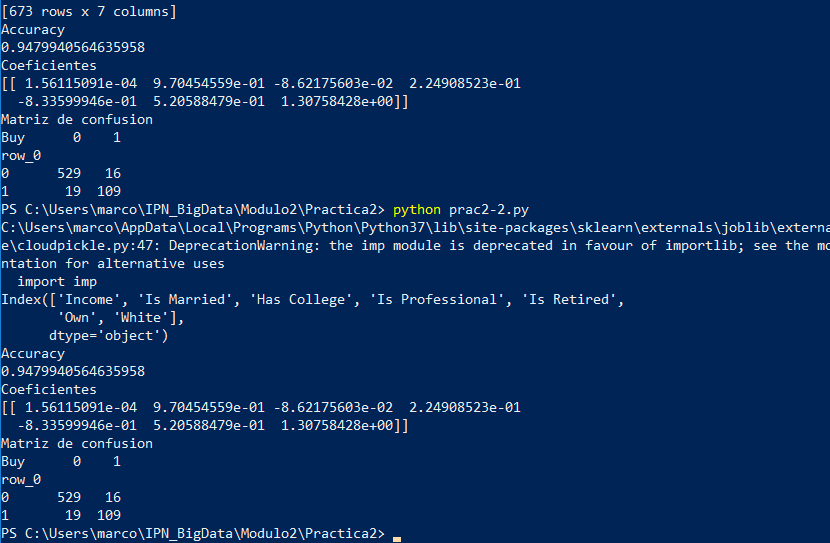
\includegraphics{resultados.png}
\end{figure}


\end{document}
